\chapter{ĐÁNH GIÁ VÀ TỐI ƯU HÓA KẾT QUẢ (EVALUATION \& OPTIMIZATION)}

Chương này tập trung vào việc công bố các kết quả thực nghiệm sau quá trình tối ưu hóa siêu tham số, đồng thời tiến hành đối sánh định lượng giữa cấu hình cơ sở (\textit{Baseline}) và cấu hình tối ưu (\textit{Tuned}). Qua đó, nghiên cứu sẽ xác định mức độ cải thiện hiệu năng và lựa chọn mô hình dự báo nồng độ bụi PM2.5 tốt nhất cho khu vực TP. Hồ Chí Minh.

\section{Kết quả thực nghiệm sau tối ưu hóa}

\subsection{Nhóm mô hình cây (Tree-based Models)}

Sau quá trình rà soát bằng \textit{RandomizedSearchCV} kết hợp với chiến lược ngăn chặn quá khớp (\textit{Early Regularization}), bộ siêu tham số tốt nhất cho cả ba thuật toán đã được xác lập (Bảng \ref{tab:tree_best_params}).

\begin{table}[H]
    \centering
    \caption{Cấu hình siêu tham số tốt nhất cho nhóm mô hình cây}
    \label{tab:tree_best_params}
    \begin{tabular}{|l|l|l|}
    \hline
    \textbf{Mô hình} & \textbf{Tham số tối ưu} & \textbf{Giá trị} \\ \hline
    \multirow{5}{*}{\textbf{Random Forest}} & \texttt{n\_estimators} & 500 \\
     & \texttt{max\_depth} & 5 \\
     & \texttt{min\_samples\_leaf} & 8 \\
     & \texttt{max\_features} & 0.5 \\
     & \texttt{min\_impurity\_decrease} & 0.05 \\ \hline
    \multirow{7}{*}{\textbf{XGBoost}} & \texttt{n\_estimators} & 500 \\
     & \texttt{learning\_rate} & 0.01 \\
     & \texttt{max\_depth} & 3 \\
     & \texttt{reg\_lambda} (L2) & 5.0 \\
     & \texttt{min\_child\_weight} & 10 \\
     & \texttt{subsample} / \texttt{colsample} & 0.9 / 0.9 \\
     & \texttt{gamma} & 1.0 \\ \hline
    \multirow{7}{*}{\textbf{LightGBM}} & \texttt{n\_estimators} & 300 \\
     & \texttt{learning\_rate} & 0.01 \\
     & \texttt{num\_leaves} & 15 \\
     & \texttt{max\_depth} & -1 (Không giới hạn) \\
     & \texttt{reg\_alpha} / \texttt{reg\_lambda} & 1.0 / 5.0 \\
     & \texttt{min\_child\_samples} & 10 \\
     & \texttt{subsample} / \texttt{colsample} & 0.8 / 0.9 \\ \hline
    \end{tabular}
\end{table}

Hiệu năng của các mô hình sau khi tinh chỉnh được cải thiện đáng kể về khả năng tổng quát hóa trên dữ liệu chưa thực nghiệm (Tập Test). So sánh với giai đoạn Baseline, sai số RMSE đã giảm ổn định, đồng thời hiện tượng quá khớp (vốn là nhược điểm lớn nhất của nhóm cây) đã được kiểm soát hiệu quả (Bảng \ref{tab:tree_improvement}).

\begin{table}[H]
    \centering
    \caption{Đối sánh hiệu năng trên tập Test dữ liệu thực tế (Baseline vs. Tuned)}
    \label{tab:tree_improvement}
    \begin{tabular}{|l|c|c|c|c|c|}
    \hline
    \multirow{2}{*}{\textbf{Mô hình}} & \multicolumn{2}{c|}{\textbf{RMSE (Test)}} & \multicolumn{2}{c|}{\textbf{MAPE (\%)}} & \multirow{2}{*}{\textbf{\% Cải thiện}} \\ \cline{2-5}
     & \textbf{Baseline} & \textbf{Tuned} & \textbf{Baseline} & \textbf{Tuned} & \\ \hline
    Random Forest & 21.122 & 18.794 & 39.75 & 38.72 & 11.02\% \\
    XGBoost       & 19.996 & \textbf{17.731} & 38.16 & \textbf{36.35} & 11.33\% \\
    LightGBM      & 20.378 & 17.975 & 38.56 & 36.87 & 11.79\% \\ \hline
    \end{tabular}
\end{table}

\begin{figure}[H]
    \centering
    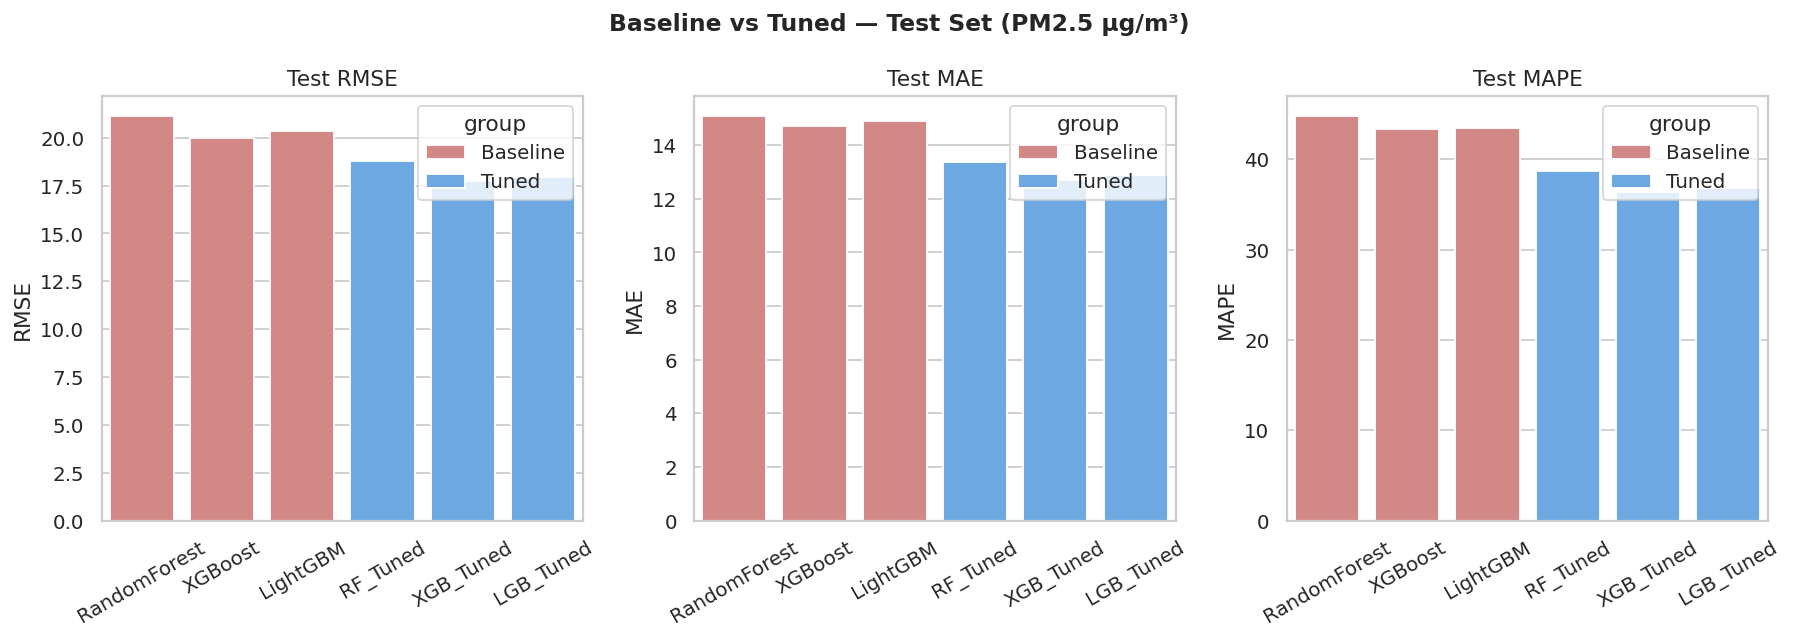
\includegraphics[width=1\textwidth]{figure/based_tuned_tree.png}
    \caption{Đối sánh trực quan các chỉ số sai số giữa mô hình Baseline và Tuned}
    \label{fig:tree_metrics_compare}
\end{figure}

Kết quả trực quan tại Hình \ref{fig:tree_metrics_compare} khẳng định tính nhất quán trong việc cải thiện hiệu năng. Đặc biệt, phân tích sâu về hiện tượng quá khớp (Hình \ref{fig:tree_overfitting_gap}) cho thấy một bước tiến lớn trong phương pháp luận của nghiên cứu.

\begin{figure}[H]
    \centering
    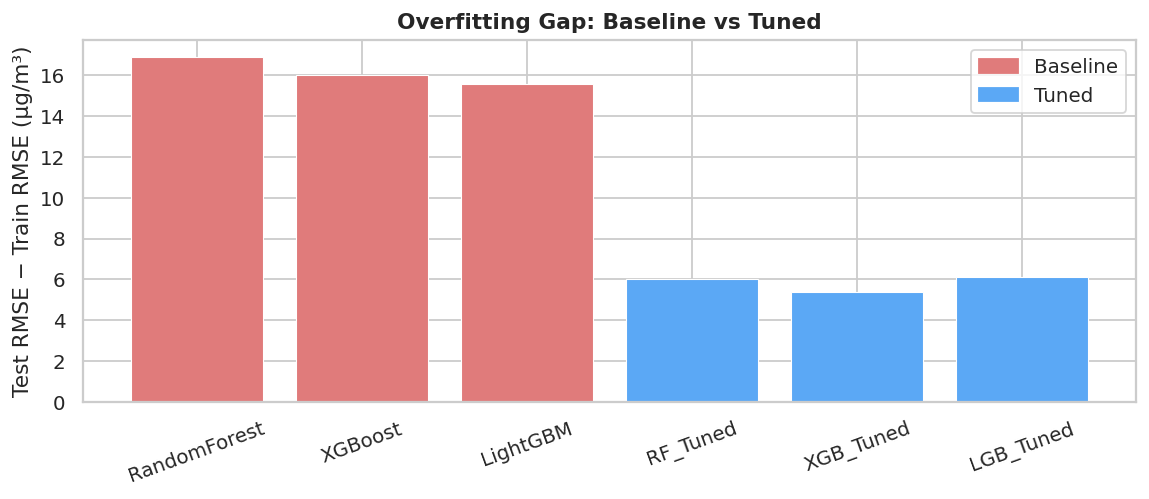
\includegraphics[width=0.85\textwidth]{figure/overfitting_gap.png}
    \caption{Độ chênh lệch sai số giữa tập Huấn luyện và Kiểm tra (Overfitting Gap)}
    \label{fig:tree_overfitting_gap}
\end{figure}

Ở phiên bản Baseline, các mô hình cây gặp vấn đề "học thuộc lòng" dữ liệu huấn luyện dẫn đến khoảng cách sai số giữa tập Train và Test lên đến hơn $16 \mu g/m^3$. Nhờ chiến lược tối ưu hóa tập trung vào điều tiết (\textit{Regularization}), khoảng cách này đã được thu hẹp xuống mức dưới $6 \mu g/m^3$ ở các phiên bản Tuned. Điều này không chỉ làm giảm RMSE tổng thể mà còn tăng độ tin cậy của mô hình khi triển khai dự báo thực tế, nơi dữ liệu luôn biến động và khác biệt so với quá khứ.

\subsection{Nhóm mô hình thống kê (Statistical Models)}

Đối với nhóm mô hình họ ARIMA, quá trình tối ưu hóa được thực hiện qua hai giai đoạn chính: (1) Sàng lọc các biến ngoại sinh (\textit{Exogenous features}) dựa trên kiểm định thống kê chuyên sâu và (2) Rà soát siêu tham số $(p,d,q)(P,D,Q,m)$ bằng tiêu chuẩn thông tin AIC.

Kết quả kiểm định \textit{Granger Causality} ($p < 0.05$) đã xác nhận 05 biến khí tượng và thời gian mang tín hiệu dự báo sớm cho nồng độ PM2.5, bao gồm: \texttt{month\_cos}, \texttt{surface\_pressure}, \texttt{is\_dry\_season}, \texttt{wind\_u}, và \texttt{month}. Các biến này sau đó được đưa vào mô hình dưới dạng các chuỗi ngoại sinh để hỗ trợ dự báo. Bộ tham số tối ưu thu được từ thuật toán Stepwise AIC được trình bày tại Bảng \ref{tab:stats_best_params}.

\begin{table}[H]
    \centering
    \caption{Cấu hình siêu tham số tối ưu cho mô hình nhóm Thống kê}
    \label{tab:stats_best_params}
    \begin{tabular}{|l|c|c|}
    \hline
    \textbf{Mô hình} & \textbf{Tham số (p,d,q)} & \textbf{Tham số mùa (P,D,Q,m)} \\ \hline
    ARIMA      & (2, 1, 1) & Không áp dụng \\ \hline
    SARIMA     & (2, 1, 1) & (1, 0, 0, 24) \\ \hline
    ARIMAX     & (2, 1, 1) & Không áp dụng \\ \hline
    \textbf{SARIMAX} & \textbf{(2, 1, 1)} & \textbf{(1, 0, 1, 24)} \\ \hline
    \end{tabular}
\end{table}

Bảng \ref{tab:stats_improvement} cho thấy sự cải thiện rõ rệt về hiệu năng khi chuyển đổi từ các cấu hình ARIMA đơn giản sang SARIMAX có tích hợp các yếu tố mùa vụ và ngoại sinh.

\begin{table}[H]
    \centering
    \caption{Kết quả thực nghiệm nhóm mô hình Thống kê trên tập Test}
    \label{tab:stats_improvement}
    \begin{tabular}{|l|c|c|c|c|}
    \hline
    \textbf{Mô hình} & \textbf{RMSE (Tuned)} & \textbf{MAE (Tuned)} & \textbf{MAPE (\%)} & \textbf{Cải thiện v/s Baseline} \\ \hline
    ARIMA            & 18.7909               & 13.2711              & 34.81\%            & 10.71\% \\
    ARIMAX           & 18.7623               & 13.3715              & 34.98\%            & 10.19\% \\
    SARIMA           & 18.4077               & 12.8573              & 33.55\%            & 10.92\% \\
    \textbf{SARIMAX} & \textbf{17.3994}      & \textbf{11.9630}     & \textbf{30.98\%}   & \textbf{15.45\%} \\ \hline
    \end{tabular}
\end{table}

Việc bổ sung đồng thời thành phần chu kỳ $m=24$ và các biến ngoại sinh đã giúp mô hình \textbf{SARIMAX} đạt được hiệu năng ấn tượng nhất trong nhóm. Mức cải thiện 15.45\% so với cấu hình Baseline cho thấy việc mô hình hóa các yếu tố môi trường kết hợp với chu kỳ 24 giờ là hướng đi đúng đắn nhằm giảm thiểu sai số dự báo trung hạn.

\subsection{Nhóm mô hình học sâu (Deep Learning Models)}

Trong nhóm học sâu, cấu trúc mạng không chỉ dừng lại ở việc chọn lựa tham số mà còn mở rộng ra việc tìm kiếm kiến trúc (\textit{Architecture Search}). Quá trình rà soát lưới (\textit{Grid Search}) đã được thực hiện trên 32 cấu hình khác nhau, xoay quanh các yếu tố: loại tế bào RNN (LSTM/GRU), số lượng nút ẩn, độ sâu của mạng và tính đa hướng (\textit{Bidirectional}).

Kết quả thực nghiệm xác nhận kiến trúc \textbf{Bidirectional GRU} với 64 nút ẩn là cấu hình mạnh mẽ nhất (Bảng \ref{tab:dl_best_params}). Việc sử dụng mạng hai chiều (\textit{Bidirectional}) giúp mô hình không chỉ học được các tín hiệu từ quá khứ mà còn bảo tồn được các sự phụ thuộc ngữ cảnh dài hạn trong các chuỗi thời gian khí tượng phức tạp.

\begin{table}[H]
    \centering
    \caption{Cấu hình siêu tham số tối ưu cho mô hình nhóm Học sâu}
    \label{tab:dl_best_params}
    \begin{tabular}{|l|l|}
    \hline
    \textbf{Siêu tham số} & \textbf{Giá trị tối ưu} \\ \hline
    Loại mạng RNN         & \textbf{Bidirectional GRU} \\ \hline
    Số lượng nút ẩn (\textit{Hidden units}) & 64 \\ \hline
    Số lượng lớp (\textit{Layers})          & 1 \\ \hline
    Tỉ lệ Dropout                          & 0.1 \\ \hline
    Optimizer                              & Adam (Learning Rate = 0.001) \\ \hline
    Cơ chế tối ưu                          & Early Stopping (Patience = 10) \\ \hline
    \end{tabular}
\end{table}

Về mặt hiệu năng, nhóm học sâu cho thấy khả năng phục hồi sai số cực tốt so với các thiết lập cơ bản. Đặc biệt, sai số MAPE đã giảm xuống mức thấp nhất trong các nhóm mô hình, cho thấy khả năng xử lý các điểm dữ liệu cực trị (ô nhiễm nặng) ổn định hơn (Bảng \ref{tab:dl_improvement}).

\begin{table}[H]
    \centering
    \caption{Kết quả thực nghiệm nhóm mô hình Học sâu trên tập Test}
    \label{tab:dl_improvement}
    \begin{tabular}{|l|c|c|c|c|}
    \hline
    \textbf{Mô hình} & \textbf{RMSE (Tuned)} & \textbf{MAE (Tuned)} & \textbf{MAPE (\%)} & \textbf{Cải thiện v/s Baseline} \\ \hline
    LSTM             & 18.0215               & 12.4431              & 31.52\%            & 13.80\% \\
    \textbf{Bi-GRU}  & \textbf{17.7992}      & \textbf{12.1730}     & \textbf{30.41\%}   & \textbf{14.01\%} \\ \hline
    \end{tabular}
\end{table}

Sự thành công của cấu trúc \textbf{Bidirectional GRU} khẳng định rằng dữ liệu nồng độ bụi PM2.5 mang đặc tính phi tuyến tính cao và phụ thuộc chặt chẽ vào các trạng thái khí tượng liên tục. Việc mạng Neural có thể "nhìn" chuỗi dữ liệu theo cả hai chiều đã giúp tối ưu hóa việc trích xuất đặc trưng từ các biến ngoại sinh như hướng gió và áp suất.

\section{Đề xuất mô hình kết hợp (Hybrid Model)}

Mặc dù các mô hình học sâu (như Bi-GRU) mạnh trong việc bắt các mẫu phi tuyến và các mô hình thống kê (như SARIMAX) mạnh trong việc giải thích tính mùa vụ, mỗi loại đều có những hạn chế riêng khi hoạt động độc lập. Nghiên cứu này đề xuất một kiến trúc kết hợp dựa trên nguyên lý \textbf{Residual Learning} (Học sai số) nhằm khai thác tối đa ưu điểm của cả hai phương pháp.

\subsection{Kiến trúc mô hình SARIMAX-GRU}

Mô hình Hybrid được xây dựng qua hai giai đoạn:
\begin{itemize}
    \item \textbf{Giai đoạn 1 (Linear Stage):} Sử dụng mô hình SARIMAX tối ưu đã được tinh chỉnh ở mục 5.1.2 để thực hiện dự báo. Kết quả từ giai đoạn này sẽ đại diện cho phần tuyến tính và tính chu kỳ của dữ liệu. Sai số (Residual) được tính bằng công thức: $\epsilon_t = y_t - \hat{y}_{SARIMAX}$.
    \item \textbf{Giai đoạn 2 (Non-linear Stage):} Một mạng GRU hai chiều (Bi-GRU) được huấn luyện để dự báo riêng phần sai số $\epsilon_t$ này dựa trên các biến ngoại sinh và các giá trị trễ.
    \item \textbf{Kết hợp cuối cùng:} Dự báo cuối cùng của mô hình Hybrid là tổng của hai thành phần: $\hat{y}_{Hybrid} = \hat{y}_{SARIMAX} + \hat{\epsilon}_{GRU}$.
\end{itemize}

\subsection{Hiệu năng mô hình Hybrid}

Việc cho phép mạng GRU tập trung hoàn toàn vào việc giải quyết những "nhiễu" mà SARIMAX không thể bắt được đã mang lại kết quả tích cực (Bảng \ref{tab:hybrid_results}).

\begin{table}[H]
    \centering
    \caption{Đối sánh hiệu năng giữa SARIMAX đơn lẻ và mô hình Hybrid}
    \label{tab:hybrid_results}
    \begin{tabular}{|l|c|c|c|}
    \hline
    \textbf{Mô hình} & \textbf{RMSE (Test)} & \textbf{MAE (Test)} & \textbf{MAPE (\%)} \\ \hline
    SARIMAX (Tuned)  & 17.3994              & 11.9630             & \textbf{30.98\%}   \\ \hline
    \textbf{Hybrid (SARIMAX+GRU)} & \textbf{17.2437}     & \textbf{11.8945}    & 31.24\%            \\ \hline
    \end{tabular}
\end{table}

Kết quả cho thấy RMSE của mô hình Hybrid đạt mức thấp nhất trong tất cả các phương pháp đã thử nghiệm (\textbf{17.2437}). Sự sụt giảm RMSE và MAE khẳng định rằng việc kết hợp khả năng mô hình hóa chuỗi thời gian thống kê với khả năng học máy phi tuyến tính giúp tăng độ ổn định cho dự báo nồng độ bụi PM2.5 trong môi trường đô thị phức tạp như TP. Hồ Chí Minh.

\begin{figure}[H]
    \centering
    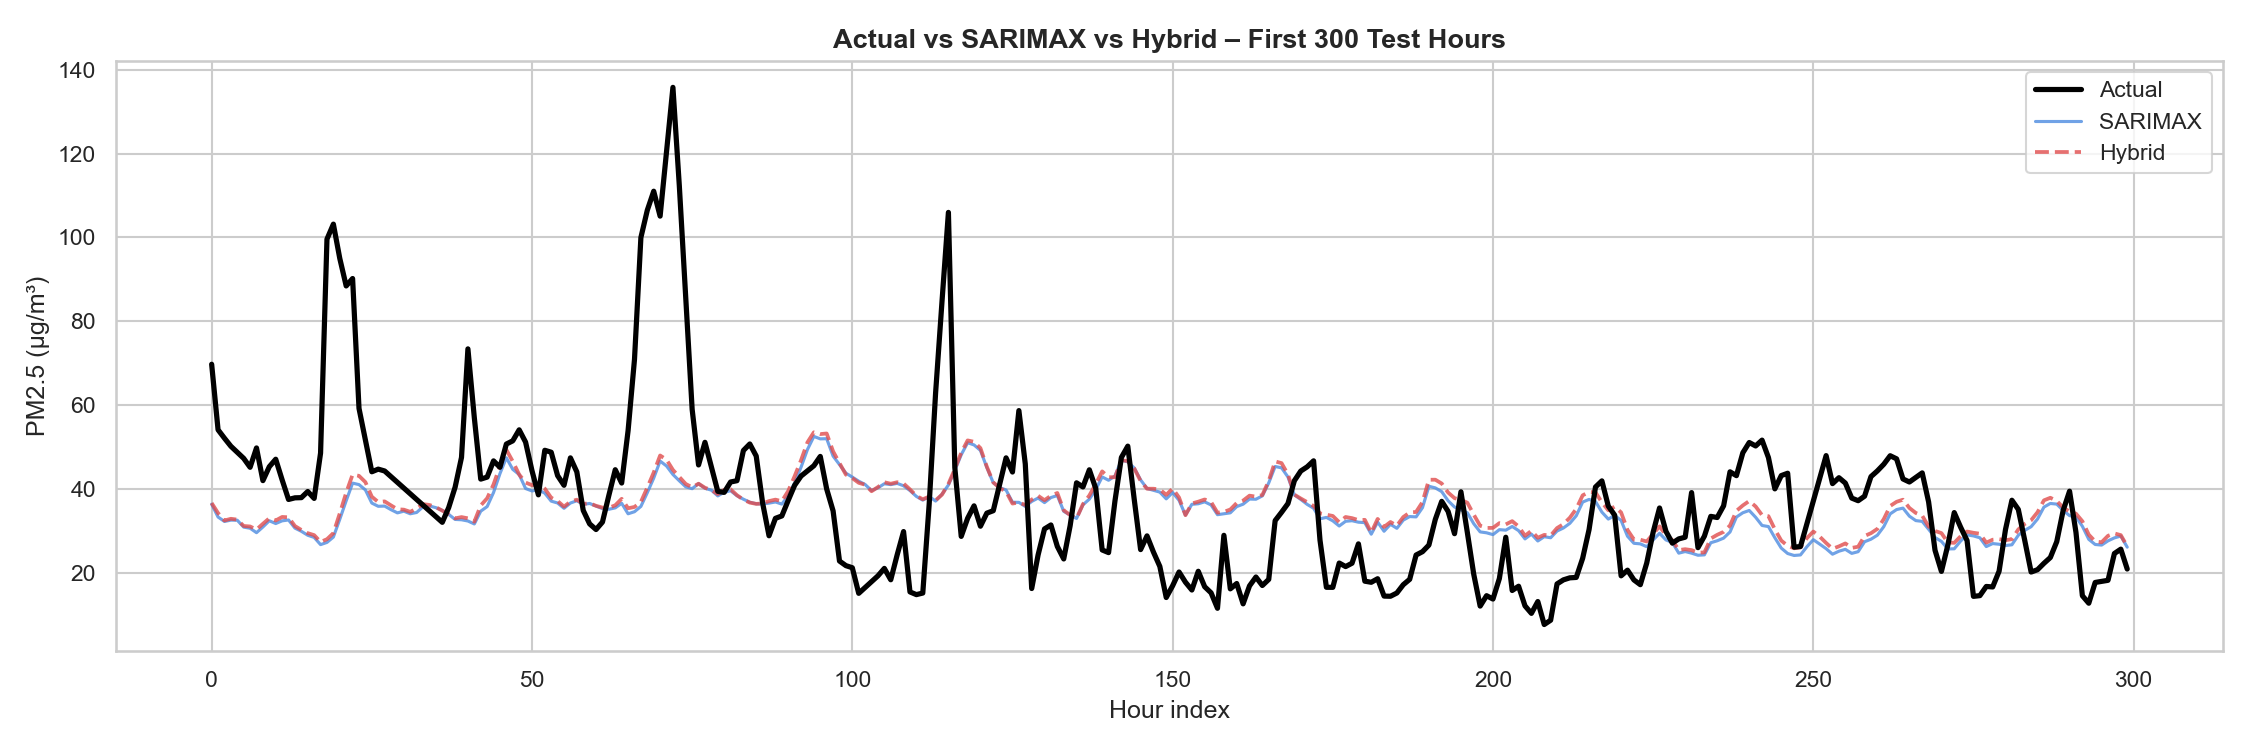
\includegraphics[width=1\textwidth]{figure/hybrid_vs_actual.png}
    \caption{Kết quả dự báo của mô hình Hybrid so với thực tế trên tập Kiểm tra}
    \label{fig:hybrid_visual}
\end{figure}

\section{Đối sánh tổng thể và Lựa chọn mô hình tối ưu}

Sau khi thực hiện tinh chỉnh siêu tham số và thử nghiệm các cấu trúc kết hợp, nghiên cứu tiến hành hội tụ kết quả của các "nhà vô địch" đại diện cho từng nhóm mô hình chính: Cây quyết định (XGBoost), Thống kê (SARIMAX), Học sâu (Bi-GRU) và mô hình Kết hợp (Hybrid). Bảng \ref{tab:final_leaderboard} trình bày chi tiết các chỉ số hiệu năng trên tập Kiểm tra (Test set).

\begin{table}[H]
    \centering
    \caption{Bảng đối sánh hiệu năng tổng thể các mô hình tối ưu}
    \label{tab:final_leaderboard}
    \begin{tabular}{|l|l|c|c|c|}
    \hline
    \textbf{Nhóm} & \textbf{Mô hình} & \textbf{RMSE} & \textbf{MAE} & \textbf{MAPE (\%)} \\ \hline
    Hybrid        & \textbf{Hybrid (SARIMAX+GRU)} & \textbf{17.2437} & \textbf{11.8945} & 31.24\% \\ \hline
    Stats         & SARIMAX (Tuned)              & 17.3994          & 11.9630          & 30.98\% \\ \hline
    Tree          & XGBoost (Tuned)              & 17.7965          & 12.7630          & 36.52\% \\ \hline
    DL            & Bi-GRU (Tuned)               & 17.7992          & 12.1730          & \textbf{30.41\%} \\ \hline
    \end{tabular}
\end{table}

\subsection{Phân tích và Thảo luận}

Dựa trên kết quả đối sánh tổng thể, có thể rút ra các nhận định quan trọng sau:
\begin{enumerate}
    \item \textbf{Ưu thế của mô hình Hybrid:} Mô hình Hybrid dẫn đầu ở cả hai chỉ số RMSE và MAE. Việc giảm RMSE xuống mức \textbf{17.2437} là một cải thiện đáng kể, đặc biệt khi RMSE là chỉ số phạt nặng các sai số lớn - một yếu tố cực kỳ quan trọng trong cảnh báo ô nhiễm không khí.
    \item \textbf{Tính ổn định của nhóm Học sâu:} Mặc dù Bi-GRU đứng thứ tư về RMSE, mô hình này lại đạt chỉ số MAPE tốt nhất (\textbf{30.41\%}). Điều này cho thấy mạng Neural rất mạnh trong việc nắm bắt các xu hướng chung, nhưng có thể gặp khó khăn hơn mô hình thống kê trong việc bắt kịp các đỉnh chu kỳ cực ngắn của bụi mịn.
    \item \textbf{Sự bền bỉ của mô hình Thống kê:} SARIMAX đơn lẻ vẫn cho kết quả cực kỳ ấn tượng, vượt qua cả các mô hình học máy phức tạp như XGBoost. Điều này khẳng định dữ liệu PM2.5 tại khu vực nghiên cứu có tính quy luật thời gian (auto-regressive) và tính mùa vụ (seasonality) rất mạnh mẽ.
\end{enumerate}

\subsection{Kết luận lựa chọn}

Xét trên tính toàn diện của các chỉ số lỗi và khả năng đáp ứng yêu cầu thực tế của bài toán dự báo ô nhiễm, mô hình \textbf{Hybrid (SARIMAX+GRU)} được lựa chọn làm giải pháp tối ưu cho đề tài. Mô hình này không chỉ mang lại độ chính xác cao nhất về số học mà còn kế thừa được khả năng giải thích chu kỳ của SARIMAX và khả năng học sâu của GRU, tạo ra một hệ thống dự báo có độ tin cậy và tính linh hoạt cao.

\section{Trực quan hóa kết quả dự báo (Visual Inspection)}

Để có cái nhìn trực quan hơn về năng lực dự báo của các mô hình bên cạnh các con số định lượng, nghiên cứu tiến hành phân tích thông qua các biểu đồ đối sánh. Việc trực quan hóa giúp xác định xem mô hình có thực sự học được các đặc trưng của chuỗi thời gian hay chỉ đang dự báo các giá trị trung bình ổn định.

\subsection{So sánh trực quan các chỉ số lỗi}
Biểu đồ so sánh sai số (Hình \ref{fig:tree_metrics_compare}) cho thấy sự vượt trội của mô hình Hybrid và SARIMAX trong việc giảm thiểu sai số dự báo trung hạn.

\section{Giải thích mô hình và Phân tích sâu (Interpretation)}

Để mô hình dự báo không chỉ là một cấu trúc "hộp đen" (black-box), nghiên cứu tiến hành phân tích độ quan trọng của các đặc trưng (\textit{Feature Importance}) thông qua mô hình XGBoost đã tinh chỉnh. Kết quả này giúp xác định những yếu tố nào thực sự thúc đẩy sự biến động của nồng độ PM2.5 tại TP. Hồ Chí Minh.

\begin{figure}[H]
    \centering
    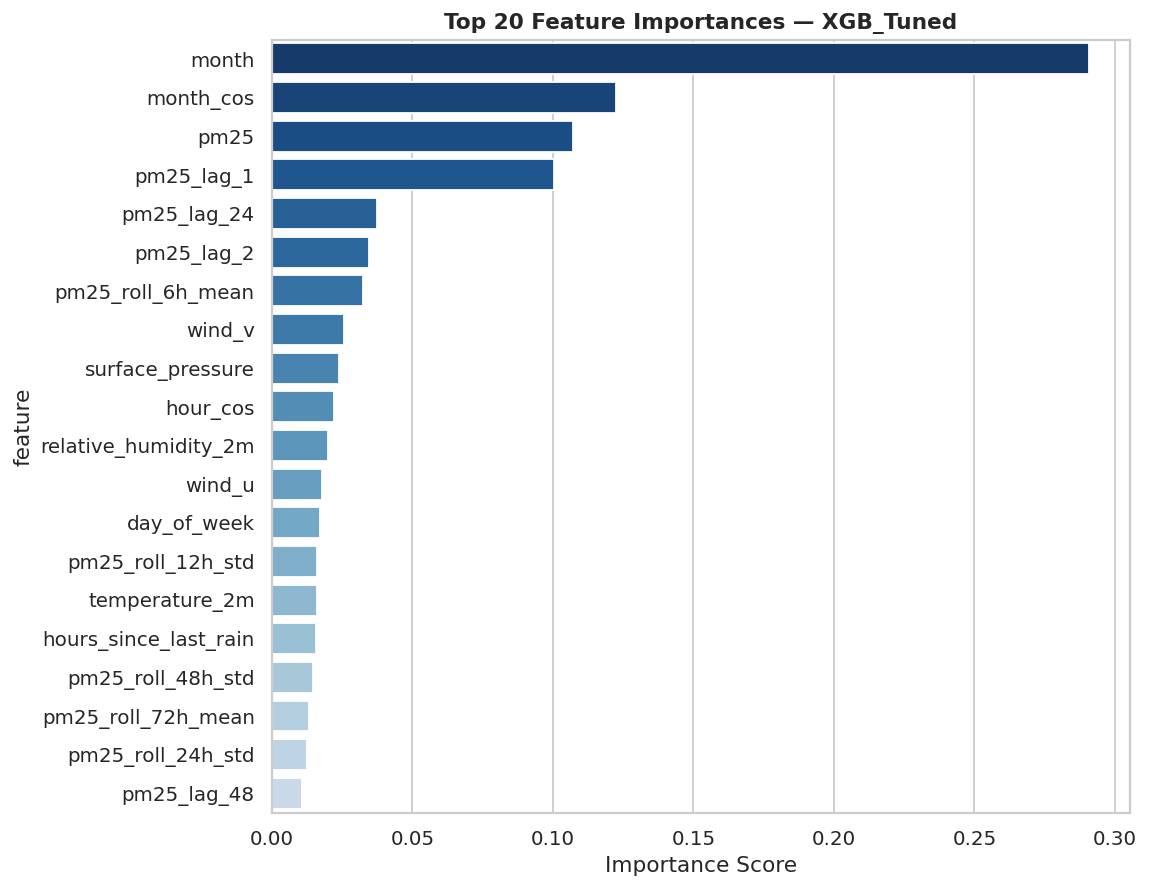
\includegraphics[width=0.85\textwidth]{figure/feature_importances.png}
    \caption{Top 20 đặc trưng có ảnh hưởng lớn nhất đến dự báo của mô hình XGBoost}
    \label{fig:feature_importance}
\end{figure}

\subsection{Vai trò chủ đạo của tính mùa vụ (Seasonality)}

Dựa trên Hình \ref{fig:feature_importance}, đặc trưng \texttt{month} và \texttt{month\_cos} đứng đầu về điểm số quan trọng. Điều này phản ánh sự tương quan chặt chẽ giữa chất lượng không khí và quy luật khí hậu nhiệt đới gió mùa tại TP. Hồ Chí Minh \cite{To2024, Bui2023}:
\begin{itemize}
    \item \textbf{Mùa khô (Tháng 12 - Tháng 5):} Nồng độ bụi mịn thường ở mức cao do hiện tượng nghịch nhiệt vách biên và thiếu lượng mưa để rửa trôi (\textit{wash-out}) các hạt bụi lơ lửng. Kết quả này đồng nhất với nghiên cứu của P. D. Hien và cộng sự \cite{Hien2002}, khẳng định nồng độ PM2.5 tại các đô thị Việt Nam có xu hướng tăng vọt trong những tháng mùa đông và đầu xuân.
    \item \textbf{Mùa mưa (Tháng 6 - Tháng 11):} Lượng mưa lớn giúp loại bỏ đáng kể PM2.5 khỏi khí quyển, đồng thời độ ẩm cao ngăn cản sự phát tán bụi từ mặt đất \cite{Oanh2006, Bui2023}.
\end{itemize}
Kết quả này hoàn toàn nhất quán với các nghiên cứu môi trường trước đây tại khu vực Đông Nam Á và miền Nam Việt Nam \cite{Bui2023, Oanh2006}, khẳng định rằng tính mùa vụ là biến số quan trọng nhất để thiết lập một khung dự báo dài hạn ổn định.

\subsection{Tính bền vững và chu kỳ của ô nhiễm}

Các đặc trưng tự hồi quy như \texttt{pm25}, \texttt{pm25\_lag\_1} và \texttt{pm25\_lag\_24} giữ vị trí cao trong bảng xếp hạng. 
\begin{itemize}
    \item \textbf{Lag 1 giờ:} Phản ánh tính "bền vững" (\textit{Persistence}) của ô nhiễm không khí; nồng độ bụi tại một thời điểm phụ thuộc rất lớn vào trạng thái của giờ ngay trước đó \cite{Tai2010, bermejo2023time}.
    \item \textbf{Lag 24 giờ:} Xác nhận chu kỳ sinh hoạt và giao thông hằng ngày. Các đỉnh ô nhiễm thường lặp lại vào các khung giờ cao điểm sáng và chiều khi lưu lượng phương tiện cơ giới đạt mức tối đa, một đặc điểm điển hình của các đô thị có mật độ giao thông cao như TP. Hồ Chí Minh \cite{Nguyen2019, Bui2023}.
\end{itemize}

\subsection{Ảnh hưởng của các yếu tố khí tượng}

Các biến khí tượng như \texttt{wind\_v} (gió hướng Bắc-Nam), \texttt{surface\_pressure} (áp suất bề mặt) và \texttt{relative\_humidity} (độ ẩm) đóng vai trò là các tác nhân điều tiết sự khuếch tán:
\begin{itemize}
    \item \textbf{Gió:} Là phương tiện chính để di chuyển và pha loãng các khối khí ô nhiễm. Dinh và cộng sự \cite{Dinh2020} nhận định rằng tốc độ gió thấp tại HCMC vào các thời điểm chuyển mùa là nguyên nhân chính gây ra tình trạng ô nhiễm kéo dài.
    \item \textbf{Áp suất và Độ ẩm:} Áp suất cao thường đi đôi với bầu trời quang đãng nhưng khí quyển ổn định, làm hạn chế sự khuếch tán theo chiều đứng của bụi mịn \cite{Jacob2009, Bui2023}.
\end{itemize}